
\documentclass[a4paper,11pt]{article}%,twocolumn
%% packages

\usepackage{blindtext} % needed for creating dummy text passages
%\usepackage{ngerman} % needed for German default language
\usepackage{amsmath} % needed for command eqref
\usepackage{amssymb} % needed for math fonts
\usepackage[colorlinks=true,breaklinks]{hyperref} % needed for creating hyperlinks in the document, the option colorlinks=true gets rid of the awful boxes, breaklinks breaks lonkg links (list of figures), and ngerman sets everything for german as default hyperlinks language
\usepackage[hyphenbreaks]{breakurl} % ben�tigt f�r das Brechen von URLs in Literaturreferenzen, hyphenbreaks auch bei links, die �ber eine Seite gehen (mit hyphenation).
\usepackage{xcolor}
\definecolor{c1}{rgb}{0,0,1} % blue
\definecolor{c2}{rgb}{0,0.3,0.9} % light blue
\definecolor{c3}{rgb}{0.3,0,0.9} % red blue
\hypersetup{
    linkcolor={c1}, % internal links
    citecolor={c2}, % citations
    urlcolor={c3} % external links/urls
}
%\usepackage{cite} % needed for cite
\usepackage[square,authoryear]{natbib} % needed for cite and abbrvnat bibliography style
\usepackage[nottoc]{tocbibind} % needed for displaying bibliography and other in the table of contents
\usepackage{graphicx} % needed for \includegraphics 
\usepackage{longtable} % needed for long tables over pages
\usepackage{bigstrut} % needed for the command \bigstrut
\usepackage{enumerate} % needed for some options in enumerate
%\usepackage{todonotes} % needed for todos
\usepackage{makeidx} % needed for creating an index
\makeindex
\usepackage{gensymb}
\usepackage{url}
\usepackage{psfrag}
\usepackage{multirow}
\usepackage{subfigure}
%% page settings

\usepackage[top=20mm, bottom=20mm,left=15mm,right=15mm]{geometry} % needed for page border settings
\parindent=0mm % for space of first line of new text block
\sloppy % for writing with hyphenless justification (tries to)
\hyphenation{} % use hyphenation of tolerance parametershttp://www.jr-x.de/publikationen/latex/tipps/zeilenumbruch.html
\hyphenpenalty=10000
\exhyphenpenalty=10000
\usepackage{fancyhdr} % needed for head and foot options
%% my macros

%% Text fomats
\newcommand{\tbi}[1]{\textbf{\textit{#1}}}

%% Math fonts
\newcommand{\bbA}{\mathbb{A}}
\newcommand{\bbB}{\mathbb{B}}
\newcommand{\bbC}{\mathbb{C}}
\newcommand{\bbD}{\mathbb{D}}
\newcommand{\bbE}{\mathbb{E}}
\newcommand{\bbF}{\mathbb{F}}
\newcommand{\bbG}{\mathbb{G}}
\newcommand{\bbH}{\mathbb{H}}
\newcommand{\bbI}{\mathbb{I}}
\newcommand{\bbJ}{\mathbb{J}}
\newcommand{\bbK}{\mathbb{K}}
\newcommand{\bbL}{\mathbb{L}}
\newcommand{\bbM}{\mathbb{M}}
\newcommand{\bbN}{\mathbb{N}}
\newcommand{\bbO}{\mathbb{O}}
\newcommand{\bbP}{\mathbb{P}}
\newcommand{\bbQ}{\mathbb{Q}}
\newcommand{\bbR}{\mathbb{R}}
\newcommand{\bbS}{\mathbb{S}}
\newcommand{\bbT}{\mathbb{T}}
\newcommand{\bbU}{\mathbb{U}}
\newcommand{\bbV}{\mathbb{V}}
\newcommand{\bbW}{\mathbb{W}}
\newcommand{\bbX}{\mathbb{X}}
\newcommand{\bbY}{\mathbb{Y}}
\newcommand{\bbZ}{\mathbb{Z}}
\usepackage[ framed, numbered]{matlab-prettifier}%framed,%
\usepackage{listings}
\usepackage{physics}
\usepackage{pdfpages}
\usepackage[toc,page]{appendix}
\usepackage{float}
% for code
\usepackage{listings}
\usepackage{color}
\usepackage{pifont}

\usepackage{scalerel,xparse}
\NewDocumentCommand\emojismile{}{
    \scalerel*{
        
\includegraphics{./figures/emoji/u1F62C.png}
    }{X}
}


% Define colors
\definecolor{codegreen}{rgb}{0,0.6,0}
\definecolor{codegray}{rgb}{0.5,0.5,0.5}
\definecolor{codepurple}{rgb}{0.58,0,0.82}
\definecolor{backcolour}{rgb}{0.95,0.95,0.92}
% Setup the listings package
\lstset{
    backgroundcolor=\color{backcolour},   
    commentstyle=\color{codegreen},
    keywordstyle=\color{magenta},
    numberstyle=\tiny\color{codegray},
    stringstyle=\color{codepurple},
    basicstyle=\footnotesize,
    breakatwhitespace=false,         
    breaklines=true,                 
    captionpos=b,                    
    keepspaces=true,                 
    numbers=left,                    
    numbersep=5pt,                  
    showspaces=false,                
    showstringspaces=false,
    showtabs=false,                  
    tabsize=2
}



\begin{document}
\begin{titlepage}
\center % Center everything on the page

%-------------------------------------------------------------------------------------
%	HEADING SECTIONS
%------------------------------------------------------------------------------------
\textbf{\large Department of Electrical and Computer Engineering}\\[0.5cm]
\textbf{\Large University of Colorado at Boulder}\\[1cm]
\textbf{\large ECEN5823 - Low Power Embedded Design Techniques}\\[2cm]

\includegraphics[width=0.3\textwidth]{figures/cu}\\[2cm] 

	
%-------------------------------------------------------------------------------------
%	TITLE SECTION
%------------------------------------------------------------------------------------
\textbf{\Huge Spring 2024, ECEN 5823 }\\[0.2cm]

\textbf{\Large Course Project Report}\\[5cm]


%----------------------------------------------------------------------------------------
%	MEMBERS SECTION
%----------------------------------------------------------------------------------------


\vfill

\textbf{\large Submitted by}

{\large Parth Thakkar}\\[0.5cm]

%----------------------------------------------------------------------------------------
%	DATE SECTION
%----------------------------------------------------------------------------------------

\textbf{\large Submitted on}\\
\textbf{\Large \today} % Date, change the \today to a set date if you want to be precise

%----------------------------------------------------------------------------------------

\vfill % Fill the rest of the page with whitespace

\end{titlepage}

\pagebreak

\tableofcontents
\listoffigures
\listoftables
\vfill
\begin{center}
    \textbf{\textit{*PDF is clickable}}
\end{center}

\pagebreak

[]{Project Proposal}
\textbf{Team name:}\\
Low Self Esteem Team\\

\textbf{Student Name:}\\
Parth Rajeshkumar Thakkar\\
ParthRajeshkumar.Thakkar@colorado.edu\\

Anagha Aditya\\
Anagha.Aditya@colorado.edu\\

Akash Karoshi\\
Akash.Karoshi@colorado.edu\\


\section{Project Overview: The Insane Keyboard}
For the ECEN 5833 Low Power Embedded System Design course, our team is developing an advanced mechanical keyboard called "The Insane Keyboard". This project aims to create a high-performance input device that combines ergonomic design, customization options, and advanced technology.
\subsection{Project Context}
Mechanical keyboards are popular for their tactile feedback and durability. However, the current market often requires users to choose between ergonomics, wireless functionality, customization, or additional features. Our project seeks to address this limitation by integrating these features into a single device.
\subsection{Project Rationale}
Our analysis of the mechanical keyboard market revealed several issues:
\begin{itemize}
    \item Ergonomic keyboards often lack additional features or are expensive
    \item Many feature-rich keyboards are wired, limiting mobility
    \item Affordable keyboards offer limited customization
    \item Few keyboards combine ergonomic design, wireless capability, programmable lighting, and smart functions
    \item Keyboards with displays or extra features often have poor power efficiency
\end{itemize}
\subsection{Project Goals}
We aim to create a mechanical keyboard with the following features:
\begin{itemize}
    \item Split ergonomic design to reduce physical strain
    \item Wireless connectivity using Bluetooth Low Energy.
    \item Programmable RGB lighting with addressable LEDs
    \item Hot-swappable key switches for easy customization
    \item Low-power E-ink display for additional information
    \item Multi-device compatibility
    \item Advanced power management techniques
    \item Environment temperature and pressure sensing.
    \item Real Time clock module for timer, stopwatch and time features.
    \item Potential energy harvesting from typing (Yet to be seen)
    \item Open-source firmware for extensive customization
    \item Cost-effective design for market accessibility
\end{itemize}

\subsection{Technical Specifications}
\begin{itemize}
    \item Microcontroller: EFR32BG13 series for low-power operation, with BLE 4/5 Stack.
    \item E-ink Display: 4.3" 800x400 E-Ink display module
    \item LED: WS2812B addressable RGB LEDs
    \item Key Switches: Compatible with Cherry MX-style switches
    \item Hot-swap Sockets: Gateron Black V2 Pro sockets
    \item Power Source: Rechargeable Li-ion battery (capacity TBD)
    \item Firmware: Based on SiLabs EFR32BG13 open-source API
\end{itemize}
\subsection{Unique Features}
"The Insane Keyboard" stands out due to its:
\begin{itemize}
    \item Integration of multiple desirable features in one device
    \item Optimized power management for extended use
    \item Potential energy harvesting from typing motions
    \item Open-source firmware for community-driven development
    \item Adaptable design for future upgrades
\end{itemize}
\subsection{Target Users}
Our keyboard is designed for:
\begin{itemize}
    \item Professionals who type for long periods
    \item Technology enthusiasts interested in customization
    \item Gamers requiring responsive keys and custom lighting
    \item Remote workers needing portable, feature-rich input devices
    \item Users seeking a versatile, high-quality keyboard
\end{itemize}
\subsection{Expected Outcomes}
Upon completion, this project could:
\begin{itemize}
    \item Set new standards for feature integration in keyboard design
    \item Improve ergonomics in daily computer use
    \item Advance keyboard power management and energy harvesting
    \item Foster a community of keyboard enthusiasts and developers
    \item Demonstrate practical applications of low-power embedded design
\end{itemize}

\subsection{Existing Products and Ideas from products}

% Placeholder for a diagram of the keyboard design
\begin{figure}[!h]
    \centering
    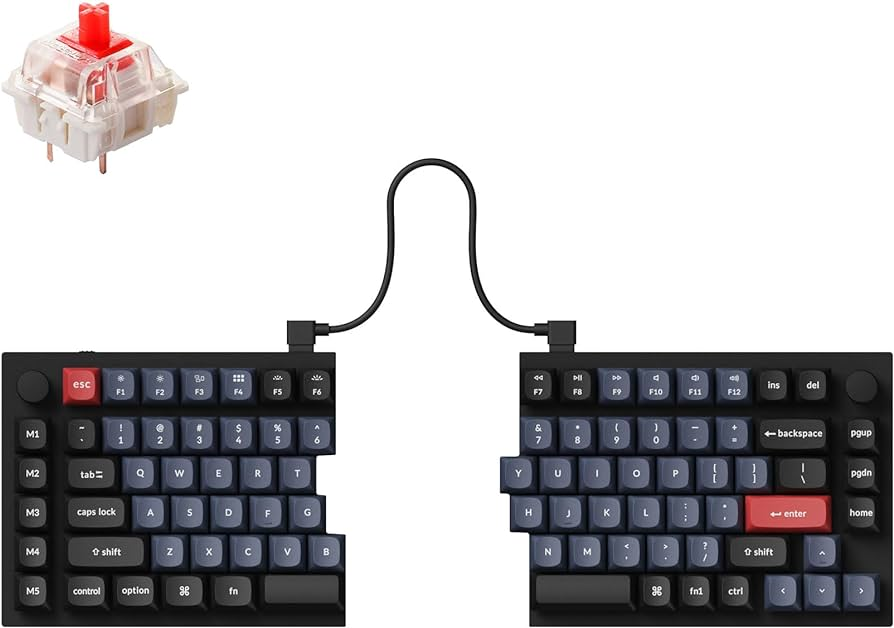
\includegraphics[scale=0.55]{figures/split_keyboard.jpg}
    \caption{Split Keyboard without display(Wired)}
    % Figure content to be added
\end{figure}
\vspace{0.2cm}
\begin{figure}[H]
    \centering
    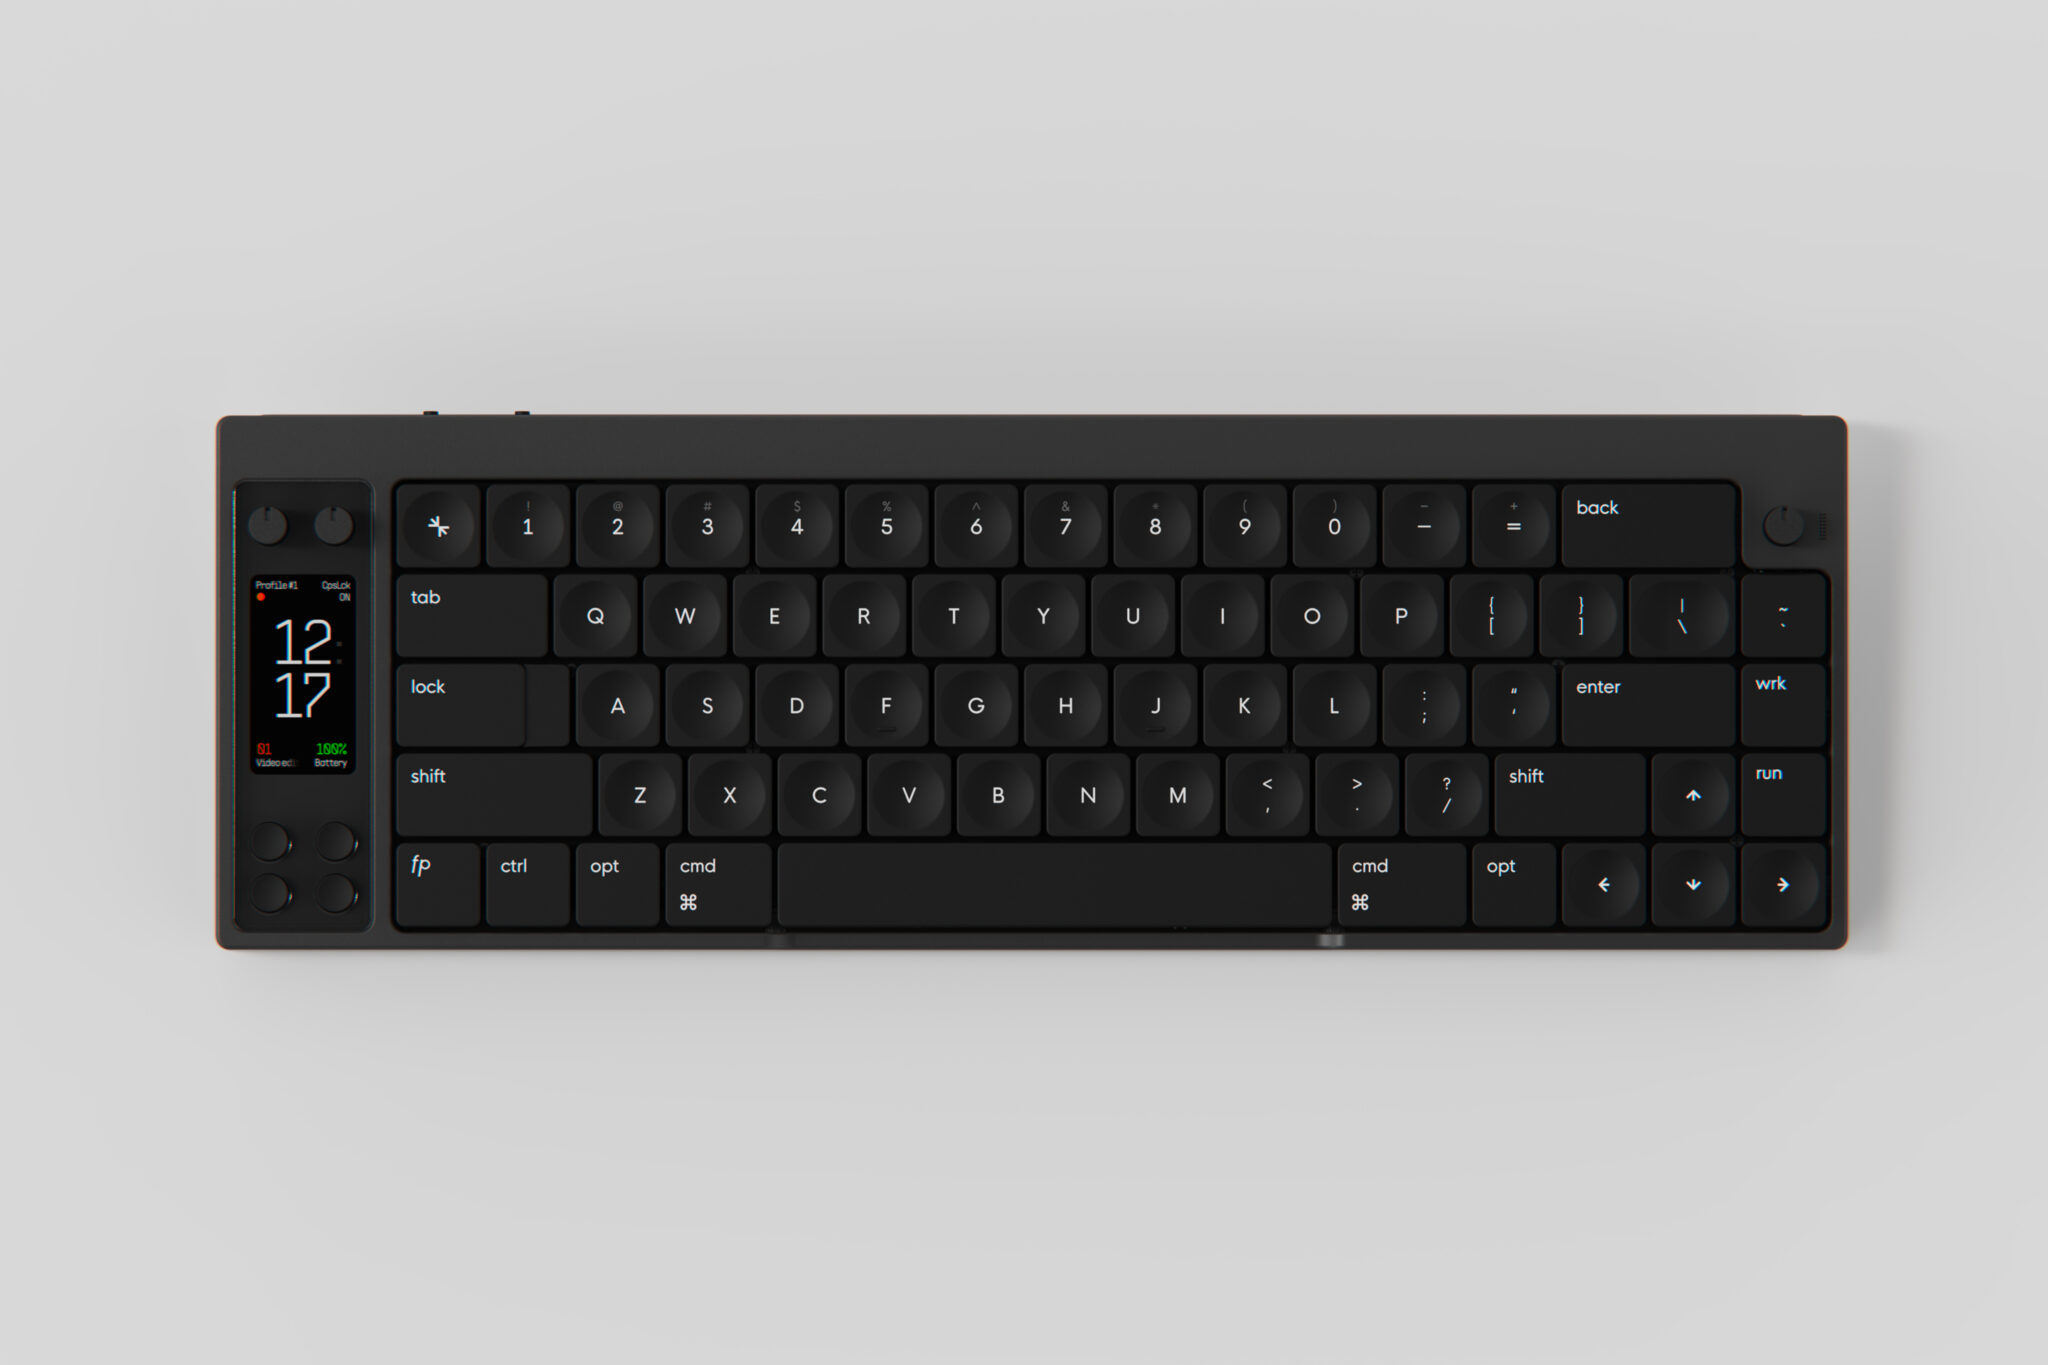
\includegraphics[scale=0.2]{figures/nomad.jpg}
    \caption{Keyboard which is expensive and have a Display}
    % Figure content to be added
\end{figure}
\vspace{0.2cm}

\begin{figure}[H]
    \centering
    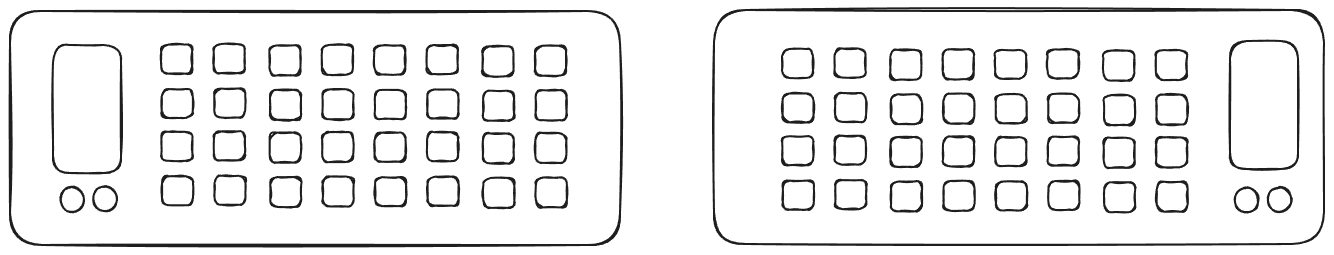
\includegraphics[scale=0.38]{figures/concept.png}
    \caption{Conceptual Design of The Insane Keyboard}
    % Figure content to be added
\end{figure}
\vspace{0.2cm}

\subsection{Project Phases}

\begin{figure}[H]
    \centering
    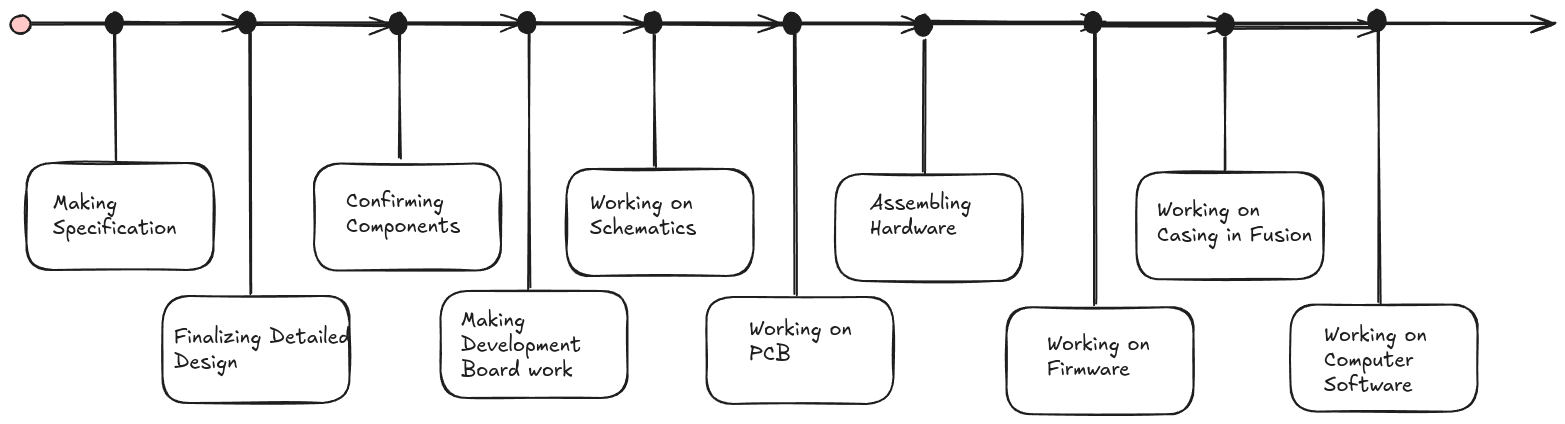
\includegraphics[scale=0.34]{figures/Timeline.png}
    \caption{Conceptual Design of The Insane Keyboard}
    % Figure content to be added
\end{figure}
\vspace{0.2cm}



\subsection{Challenges and Considerations}

Managing state machines with complex softwares like eink Display
Making drivers inegrate with BLE firmware
RTC driver and tempurature control driver 
Ensuring reliable wireless Connectivity
Multi-host communication, multi-host switching
HID Profile in BLE stack 
Anti ghosting 
making scan rate of keyboard fast enough for low latency
N-Key rollover/ 6-key rollover



\section{High Level Requirements}

\subsection{SubModules}

the board will have these modules which we will refer through out the Report

1) Main board (will have one EFR32BG13 , one display, keys )
main board will have following keys 
- (esc ~,`), (f1, 1, !), (f2, 2, @), (f3, 3, \#), (f4, 4, \$), (f5, 5, \%), (f6, 6, \^)
- Tab, Q, W, E, R, T,
- Cap, A, S, D, F, G
- Shift, Z, X, C, V, B
- CTRL, Option, Win/Mac, ALT, SPACE
- Two knobs, 3 extra buttons 
- one e ink display

Battery, Battery charging unit.

2) Secondary module will have one EFM32BG13, one display, and secondary board will have following things
- F7, F8, F9, F10, F11, F12, backspace, home
- Y, U, I , P, {[, ]}, |\\, Del
- H, j, K, L, ;:, "', enter, pageup
- N, M, , ,<, .>, /?, shift up arrow, page down
- space, alt/mac, fn, ctrl, left, down, right arrow
- Two knobs, 3 extra buttons
- one eink display

\subsection{Requirements}

-> whole product will have two EFR32BG13 Boards
-> Server will be our keyboard
-> it will be 75\% layout
-> It will have io expander for each mcu
-> It should have tempureature sensor 
-> it should have pressure sensor
-> it should have RTC
-> it should connect to three host
-> it should have one computer software to customize LED
-> each led will be individually Customizable
-> each part of the keyboard will have an e ink display
-> each part of keayboard will have energy harvesring 
-> each part of keyboard will have charging circuit and to charge both the device we will plug in type c cable to one device and other device will be conectted to chargin device via some + and - pins to bridge both the device 
-> it should have chargin indicator
-> it should have battery indicator 
-> it should have atlease 6key rollover 
-> Both EFR32BG13 board will comminicate via HID protocol one board will be connected to main board via some protocol and main board will 
\subsection{Components}

\subsection{Requirements Completion}
Section Author: Parth Thakkar\\\\

\begin{table}[H]
    \centering
    \begin{tabular}{| l | c |   }
        \hline
        \textbf{Requirements}                                                         & \textbf{Completion} \\\hline
        The system shall comprise a pair of EFR32BG13                                 & \ding{52}           \\
        \hline
        Server shall host an MFRC522 RFID reader module and a rotary encoder.         & \ding{52}           \\
        \hline
        The server shall employ Huffman encoding for data compression.                & \ding{52}           \\\hline
        The server shall establish a secure connection through bonding.               & \ding{52}           \\\hline
        The server code shall be optimized for low energy consumption.                & \ding{52}           \\\hline
        The client shall receive the compressed authentication data from the server.  & \ding{52}           \\\hline
        The Server shall display the authentication and other information on the LCD. & \ding{52}           \\\hline
        client decompress the received data using Huffman decoding                    & \ding{55}           \\\hline
        \hline\hline
    \end{tabular}
    \caption{Requirements}
    \label{filterspecs}
\end{table}

-> EFR32BG13  https://www.silabs.com/mcu/32-bit-microcontrollers/efm32pg23-series-2
-> ds3231 - RTC module - https://www.analog.com/media/en/technical-documentation/data-sheets/ds3231.pdf - I2C
-> ds3231 - RTC module breakout board - https://www.adafruit.com/product/3013
-> IO expander - I2C
-> Wave share e-ink display - https://www.waveshare.com/4.2inch-e-paper-module.htm - SPI
-> TMP117 - Tempurature and Humidity sensor - https://www.ti.com/lit/ds/symlink/tmp117.pdf?ts=1725195107763 - I2C
-> Diodes
-> Gateron Black keys
-> cherry mx key caps
-> che


2. Features and Specifications
The Insane Keyboard is designed to be a feature-rich, highly customizable input device that pushes the boundaries of what's possible in keyboard technology. This section provides a detailed breakdown of its features and specifications.
2.1 High-Level Features
2.1.1 Mechanical Key Switches

Type: Gateron switches (multiple options for user choice)
Characteristics:

Tactile feedback
Durability rated for 50 million keystrokes
Various actuation forces available (e.g., 45g, 55g, 65g)



2.1.2 Ergonomic Split Design

Two separate keyboard halves for optimal positioning
Tenting mechanism for wrist comfort (adjustable angles: 0°, 5°, 10°)
Palm rests with memory foam for extended typing comfort

2.1.3 Hot-Swappable Key Switches

Socket type: Kailh hot-swap sockets
Compatibility: Cherry MX-style switches and clones
Tool-free switch replacement for easy customization

2.1.4 Customizable RGB Lighting

Per-key RGB LEDs (16.8 million colors)
Customizable lighting patterns and effects
Brightness control: 0-100% in 5% increments
Power-efficient LED driver for extended battery life

2.1.5 Wireless Connectivity

Primary wireless technology: Bluetooth 5.0
Secondary option: 2.4GHz wireless with USB dongle
Range: Up to 10 meters (33 feet)
Latency: <1ms in 2.4GHz mode, <20ms in Bluetooth mode

2.1.6 Multiple Host Connectivity

Support for up to 3 devices simultaneously
Fast switching between devices (< 500ms)
Compatible with Windows, macOS, Linux, iOS, and Android

2.1.7 Anti-Ghosting and Anti-Aliasing

N-key rollover (NKRO) over USB and 6-key rollover over wireless
Advanced firmware algorithms for accurate key detection

2.1.8 E-ink Display

Size: 2.13" diagonal
Resolution: 250 x 122 pixels
Refresh rate: Partial refresh at 5Hz, full refresh at 1Hz
Content: Time, date, battery status, current profile, custom graphics

2.1.9 Wired Operation

USB Type-C port for charging and wired mode
USB 2.0 data transfer in wired mode

2.1.10 Integrated Applications

Spotify integration for music control and now-playing information
Customizable timer and stopwatch functions
Ability to display custom graphics/logos on the E-ink display

2.1.11 Advanced Power Management

Smart power states (active, idle, deep sleep)
Configurable auto-sleep timers
Low battery alerts and power-saving mode

2.1.12 Energy Harvesting

Kinetic energy harvesting from key presses
Supplementary power source to extend battery life

2.1.13 Temperature Monitoring

Built-in temperature sensor for device health monitoring
Thermal throttling to prevent overheating

2.2 Components
2.2.1 Main Controllers

Model: 2x Blue Gecko EFM32BG13
Features:

ARM Cortex-M4 core
512KB Flash, 64KB RAM
Built-in Bluetooth radio
Ultra-low power modes



2.2.2 Key Switches

Brand: Gateron
Types available: Blue (clicky), Brown (tactile), Red (linear)
Lifespan: 50 million keystrokes

2.2.3 IO Expander

Model: TCA9555 I2C I/O expander
Features: 16 GPIO pins for matrix scanning

2.2.4 E-ink Displays

Model: 2x Waveshare 2.13" E-Ink display module
Controller: SSD1675
Interface: SPI

2.2.5 Batteries

Type: Li-Ion 18650
Capacity: 3000mAh each (one per keyboard half)
Expected battery life: Up to 3 months with typical usage

2.2.6 Temperature Sensors

Model: TMP102
Accuracy: ±0.5°C
Interface: I2C

2.2.7 Power Management Unit (PMU)

Model: BQ25120A
Features:

Integrated battery charger
Low quiescent current: 600nA
Programmable charge current: 5mA to 300mA



2.2.8 RGB LED Driver

Model: IS31FL3733
Features:

192 LED driver channels
Built-in PWM generator
I2C interface for control



2.2.9 Energy Harvesting Module

Model: LTC3588-1
Features:

Ultra-low quiescent current: 950nA
Integrated full-wave bridge rectifier



2.3 Technical Specifications
2.3.1 Keyboard Layout

75\% layout (84 keys)
Split design (42 keys per half)
Additional function layer accessible via Fn key

2.3.2 Dimensions

Each half: 160mm x 150mm x 40mm (L x W x H)
Weight: Approximately 450g per half

2.3.3 Connectivity

Bluetooth 5.0
2.4GHz wireless (with included USB dongle)
USB Type-C for wired mode and charging

2.3.4 Power Consumption

Active mode (with backlighting): ~100mA
Active mode (without backlighting): ~30mA
Idle mode: ~5mA
Deep sleep mode: <100µA

2.3.5 Compatibility

Operating Systems: Windows 7+, macOS 10.12+, Linux, iOS 13+, Android 8.0+
Supported Bluetooth profiles: HID, HOGP


3. Software Architecture
The software architecture for the Insane Keyboard is designed to be modular, extensible, and efficient. It consists of two main components: the firmware running on the keyboard itself and the host software for customization. This section provides a detailed overview of both components.
3.1 Firmware Stack
The firmware is the core software running on the Blue Gecko EFM32BG13 controllers. It's responsible for handling all the low-level operations of the keyboard.
3.1.1 Operating System

RTOS: FreeRTOS

Provides real-time multitasking capabilities
Efficient task scheduling and inter-task communication
Low memory footprint suitable for embedded systems



3.1.2 Bluetooth Stack

Bluetooth LE Stack: Silicon Labs Bluetooth SDK

Implements Bluetooth 5.0 protocol
Supports multiple connections for host switching
Includes power-efficient connection parameters



3.1.3 USB Stack

USB Implementation: Silicon Labs USB stack

Supports USB HID class for keyboard functionality
Implements USB CDC for firmware updates



3.1.4 Key Scanning and Debouncing

Custom implementation using hardware timers and interrupts
Efficient matrix scanning algorithm
Advanced debouncing technique to prevent ghosting and improve responsiveness

3.1.5 LED Control Module

PWM-based RGB LED control
Supports various lighting effects (static, breathing, wave, etc.)
Power-efficient implementation with dimming capabilities

3.1.6 Power Management Module

Implements different power states (active, idle, sleep)
Handles transitions between power states based on user activity and battery level
Integrates with energy harvesting system for optimal power usage

3.1.7 E-ink Display Driver

SPI-based communication with E-ink display controller
Implements partial and full refresh modes
Manages display content updates (time, battery status, custom graphics)

3.1.8 Configuration Management

Stores user preferences in non-volatile memory
Manages multiple keyboard profiles
Handles firmware updates

3.1.9 Inter-Keyboard Communication

Implements custom protocol for communication between keyboard halves
Ensures synchronization of key states and LED effects

3.1.10 Sensor Integration

Reads and processes data from the temperature sensor
Implements thermal management algorithms

3.1.11 API Layer

Provides a unified interface for host software to interact with keyboard features
Implements secure communication protocol for configuration changes

3.2 Host Software
The host software runs on the user's computer and provides an intuitive interface for keyboard customization.
3.2.1 Development Framework

Framework: Kivy (Python-based)

Cross-platform compatibility (Windows, macOS, Linux)
Rich UI capabilities for an intuitive user experience



3.2.2 Core Modules
3.2.2.1 Connection Manager

Handles discovery and connection to the keyboard
Manages multiple connection types (Bluetooth, 2.4GHz wireless, USB)

3.2.2.2 Key Mapping Editor

Visual interface for remapping keys
Supports multiple layers and complex key combinations
Implements macro recording and editing

3.2.2.3 RGB Lighting Configurator

Visual tool for creating and editing lighting effects
Supports per-key RGB configuration
Provides a library of preset effects and the ability to create custom ones

3.2.2.4 Profile Manager

Allows creation, editing, and deletion of keyboard profiles
Supports import/export of profiles for sharing

3.2.2.5 Firmware Updater

Checks for and applies firmware updates
Provides rollback capability in case of update failures

3.2.2.6 E-ink Display Customizer

Interface for customizing E-ink display content
Supports uploading custom graphics and configuring display layouts

3.2.2.7 Power Management Interface

Displays battery status and power consumption statistics
Allows configuration of power-saving features

3.2.2.8 Diagnostic Tools

Provides keyboard health information (e.g., switch actuation counts, temperature readings)
Offers troubleshooting and calibration tools

3.2.3 Spotify Integration Module

Implements Spotify Web API for music control and now-playing information
Manages OAuth authentication for secure access to user's Spotify account

3.2.4 Cloud Sync Module (Future Extension)

Will allow syncing of profiles and settings across multiple devices
Planned implementation using a secure cloud storage solution

3.3 Development Approach
3.3.1 Firmware Development

Language: C
IDE: Simplicity Studio (Silicon Labs' integrated development environment)
Version Control: Git with GitLab for collaborative development
Testing: Unit testing with Unity framework, integration testing on actual hardware

3.3.2 Host Software Development

Language: Python
IDE: PyCharm
Version Control: Git with GitLab
Testing: Unit testing with pytest, UI testing with Kivy's built-in test suite

3.3.3 Continuous Integration/Continuous Deployment (CI/CD)

Automated build and test processes using GitLab CI
Nightly builds with automated smoke tests
Automated generation of firmware packages and host software installers

3.4 Security Considerations

Implement secure boot to prevent unauthorized firmware modifications
Use encryption for all wireless communications (Bluetooth and 2.4GHz)
Implement secure storage for sensitive information (e.g., Spotify tokens)
Regular security audits and penetration testing

3.5 Future Extensibility
The software architecture is designed with future extensibility in mind:

Modular design allows easy addition of new features
API-driven approach enables third-party integrations
Open-source release of host software to encourage community contributions

This comprehensive software architecture ensures that the Insane Keyboard not only meets its current feature requirements but also provides a solid foundation for future enhancements and community-driven development.


4. Hardware Design
The hardware design of the Insane Keyboard is crucial to achieving our goals of ergonomics, functionality, and energy efficiency. This section provides a detailed overview of the hardware components, design considerations, and manufacturing process.
4.1 PCB Design
4.1.1 Layout

Split design with two identical PCBs (one for each half)
4-layer PCB for optimal signal integrity and EMI reduction
Dimensions: 160mm x 150mm per half

4.1.2 Key Features

Hot-swappable switch sockets (Kailh or equivalent)
Per-key RGB LED placement
Dedicated controller section with proper isolation
High-speed and low-speed sections separated for signal integrity

4.1.3 Power Design

Separate power planes for digital and analog sections
Low-dropout regulators for clean power to sensitive components
Power filtering for RF sections (Bluetooth and 2.4GHz)

4.1.4 Signal Integrity

Controlled impedance traces for high-speed signals
Ground plane stitching to reduce EMI
Proper decoupling capacitor placement

4.1.5 Design Software

Altium Designer for schematic capture and PCB layout
SolidWorks for 3D modeling of PCB and components

4.1.6 Design for Manufacturing (DFM)

Adherence to PCB manufacturer's design rules
Panelization for efficient production
Fiducial markers for automated assembly

4.2 Key Switch Integration
4.2.1 Switch Compatibility

Support for Cherry MX-style switches and clones
Hot-swappable sockets for tool-free switch replacement

4.2.2 Mechanical Considerations

Reinforced mounting points to prevent PCB flex
Alignment pins for precise switch positioning

4.2.3 Electrical Integration

ESD protection on switch connections
Optimized trace routing for minimal latency

4.3 Microcontroller Integration
4.3.1 Blue Gecko EFM32BG13 Integration

Proper power supply decoupling
Crystal oscillator design for precise timing
Programming and debug interface accessibility

4.3.2 Peripheral Connections

I2C bus for connecting sensors and LED drivers
SPI interface for E-ink display
USB interface with ESD protection

4.4 Wireless Connectivity
4.4.1 Bluetooth Antenna Design

Integrated PCB antenna for Bluetooth
Impedance matching network for optimal performance
Keep-out zones around antenna for interference reduction

4.4.2 2.4GHz Proprietary Radio

Separate antenna for 2.4GHz communication
RF shielding to minimize interference

4.5 Power Management
4.5.1 Battery Integration

Battery holder design for easy replacement
Protection circuitry (over-voltage, under-voltage, over-current)
Fuel gauge integration for accurate battery level monitoring

4.5.2 Charging Circuit

USB Type-C connector for charging and data
Efficient charging IC with programmable charging profiles
Thermal management for safe charging

4.5.3 Energy Harvesting

Integration of piezoelectric elements under key switches
Energy harvesting IC (e.g., LTC3588-1) for power conditioning
Storage capacitors for harvested energy

4.6 E-ink Display Integration
4.6.1 Mounting

Secure mounting solution for E-ink display module
Shock and vibration resistance considerations

4.6.2 Connections

Flexible PCB connection to main board
Proper shielding for data lines

4.7 Ergonomic Considerations
4.7.1 Split Design

Adjustable tenting mechanism (0°, 5°, 10°)
Magnetic coupling system for optional attachment of halves

4.7.2 Wrist Rest

Detachable memory foam wrist rest
Durable, easy-to-clean surface material

4.8 Enclosure Design
4.8.1 Material Selection

High-quality ABS plastic for main body
Aluminum base plate for rigidity and weight

4.8.2 Manufacturing Process

Injection molding for plastic components
CNC machining for metal components

4.8.3 Aesthetic Considerations

Minimalist design with clean lines
Customizable top plate options (different colors/materials)

4.8.4 Functional Design

Proper ventilation for heat dissipation
Cable routing channels for clean setup
Non-slip feet for stability

4.9 Assembly and Manufacturing
4.9.1 PCB Assembly

Automated SMT assembly for most components
Manual assembly for through-hole components (e.g., hot-swap sockets)
Comprehensive in-circuit testing (ICT) for quality assurance

4.9.2 Final Assembly

Modular assembly process for easy customization
Comprehensive functional testing of each unit
Quality control checks at each stage of assembly

4.9.3 Packaging

Custom-designed packaging for protection during shipping
Eco-friendly materials for sustainability

4.10 Prototyping and Testing
4.10.1 Prototyping Stages

Breadboard prototypes for initial circuit validation
3D printed enclosure prototypes for ergonomic testing
Small batch PCB prototypes for full functional testing

4.10.2 Testing Procedures

Automated key switch testing rig
RF anechoic chamber testing for wireless performance
Environmental testing (temperature, humidity, drop tests)
EMC pre-compliance testing

4.11 Certifications and Compliance

FCC certification for wireless devices
CE marking for European market
RoHS compliance for environmental safety
Bluetooth SIG certification

4.12 Future Hardware Considerations

Exploration of alternative materials (e.g., recycled plastics)
Investigation of more efficient energy harvesting technologies
Potential integration of haptic feedback systems
Consideration of modular add-on capabilities

This comprehensive hardware design ensures that the Insane Keyboard not only meets its current feature requirements but also provides a solid foundation for future enhancements and iterations. The focus on quality, ergonomics, and sustainability aligns with our goal of creating a premium, long-lasting product.

\subsubsection{Wireless Communication Details / Data types}



\textbf{Object Transfer Service for RFID}
\begin{enumerate}
    \item Object Transfer Service (OTS) for RFID Data:\\
          Service UUID: 1825\\
          Service Name: "Object Transfer Service"
    \item Characteristics for Object Transfer Service: a. OTS Feature Characteristic:\\
          Characteristic UUID: 2ABD\\
          Characteristic Name: "OTS Feature"\\
          Characteristic Properties: Read\\
          Characteristic Value:\\
          Data Type: Unsigned Integer (32-bit)\\
          Length: 4 bytes\\
          Description: This characteristic indicates the features supported by the OTS server.
    \item Object Name Characteristic:\\
          Characteristic UUID: 2ABE\\
          Characteristic Name: "Object Name"\\
          Characteristic Properties: Read\\
          Characteristic Value:\\
          Data Type: UTF-8 String\\
          Length: Variable\\
          Description: This characteristic holds the name of the RFID object being transferred.\\
    \item Object Type Characteristic:\\
          Characteristic UUID: 2ABF\\
          Characteristic Name: "Object Type"\\
          Characteristic Properties: Read\\
          Characteristic Value:\\
          Data Type: UUID (128-bit)\\
          Length: 16 bytes\\
          Description: This characteristic indicates the type of the RFID object being transferred.\\
    \item Object Size Characteristic:\\
          Characteristic UUID: 2AC0\\
          Characteristic Name: "Object Size"\\
          Characteristic Properties: Read\\
          Characteristic Value:\\
          Data Type: Unsigned Integer (32-bit)\\
          Length: 4 bytes\\
          Description: This characteristic holds the size of the RFID object being transferred.\\
    \item Object Properties Characteristic:\\
          Characteristic UUID: 2AC1\\
          Characteristic Name: "Object Properties"\\
          Characteristic Properties: Read\\
          Characteristic Value:\\
          Data Type: Unsigned Integer (32-bit)\\
          Length: 4 bytes\\
          Description: This characteristic indicates the properties of the RFID object being transferred.
    \item Object Action Control Point Characteristic:
          Characteristic UUID: 2AC2\\
          Characteristic Name: "Object Action Control Point"\\
          Characteristic Properties: Write\\
          Characteristic Value:\\
          Data Type: Unsigned Integer (8-bit)\\
          Length: 1 byte\\
          Description: This characteristic is used to control the transfer of the RFID object.
    \item Object Action Control Point Response Characteristic:\\
          Characteristic UUID: 2AC3\\
          Characteristic Name: "Object Action Control Point Response"\\
          Characteristic Properties: Notify\\
          Characteristic Value:\\
          Data Type: Unsigned Integer (8-bit)\\
          Length: 1 byte\\
          Description: This characteristic provides the response to the Object Action Control Point commands.
    \item Object List Control Point Characteristic:\\
          Characteristic UUID: 2AC4\\
          Characteristic Name: "Object List Control Point"\\
          Characteristic Properties: Write\\
          Characteristic Value:\\
          Data Type: Unsigned Integer (8-bit)\\
          Length: 1 byte\\
          Description: This characteristic is used to control the listing of RFID objects.
    \item Object List Control Point Response Characteristic:
          Characteristic UUID: 2AC5\\
          Characteristic Name: "Object List Control Point Response"\\
          Characteristic Properties: Notify\\
          Characteristic Value:\\
          Data Type: Unsigned Integer (8-bit)\\
          Length: 1 byte\\
          Description: This characteristic provides the response to the Object List Control Point commands.\\
    \item Object Changed Characteristic:\\
          Characteristic UUID: 2AC6\\
          Characteristic Name: "Object Changed"\\
          Characteristic Properties: Indicate\\
          Characteristic Value:\\
          Data Type: Boolean\\
          Length: 1 byte\\
          Description: This characteristic indicates whether the RFID object has changed.\\
\end{enumerate}


\pagebreak
\subsubsection{Functional hardware block diagram}

hardware block diagram illustrates the components and connections of the RFID-based authentication system. At the top, the RFID reader and rotary encoder are shown as input devices connected to the server, which is an EFR32BG13 board. The server board processes the data from these input devices and applies Huffman encoding for data compression. The compressed data is then transmitted via Bluetooth Low Energy (BLE) to the client, which is another EFR32BG13 board. The client board receives the encoded data, decodes it using Huffman decoding, and performs authentication checks. The authentication status is displayed on an LCD connected to the client board, and if the authentication is successful, an LED is turned on, and a servo motor is activated. The diagram provides a clear overview of the main components and the flow of data within the RFID-based authentication system.

% \begin{figure}[H]
% 	\centering
% 	\includegraphics[scale=0.6]{figures/hwblcodiagram.png}
% 	\caption{Hardware block diagram}
% 	\label{idealbpfilter}
% \end{figure}

\subsubsection{Functional software block diagram}


software block diagram illustrates the components and flow of the RFID-based authentication system. At the center, the Event Handler acts as the core component, receiving events from the BLE stack, Object Transfer Service, and Custom Service. The BLE stack handles the Bluetooth Low Energy communication, while the Huffman Encoding block is responsible for compressing and decompressing data. The LCD UI interacts with the Event Handler to display relevant information to the user. The Event Handler communicates with the RFID reader and rotary encoder through their respective drivers, which are implemented using SPI (Serial Peripheral Interface) and GPIO interrupts. The RFID driver reads the RFID tag data, while the rotary encoder driver captures the user input from the rotary encoder. The Event Handler processes the received data and triggers appropriate actions, such as sending data over BLE or updating the LCD UI. Overall, this software architecture enables efficient handling of events, data compression, and communication between the various components of the RFID-based authentication system

% \begin{figure}[H]
% 	\centering
% 	\includegraphics[scale=0.38]{figures/sw_block_diagram_client.png}
% 	\caption{Software Block diagram For Client}
% 	\label{idealbpfilter}
% \end{figure}

% \begin{figure}[H]
% 	\centering
% 	\includegraphics[scale=0.38]{figures/swblockdiagram_server.png}
% 	\caption{Software Block diagram For Server}
% 	\label{idealbpfilter}
% \end{figure}

\subsubsection{Energy modes}


Gecko remains in EM3 (Sleep Mode) until an RFID tag is detected or the rotary encoder is rotated, which triggers a wake-up event. Upon wake-up, the system enters EM0 (Active Mode) to process the authentication data, perform data compression, and send BLE notifications. After completing the necessary tasks, the system goes back to EM3 to conserve power until the next wake-up event occurs.

% \begin{figure}[H]
% 	\centering
% 	\includegraphics[scale=0.32]{figures/energymode.png}
% 	\caption{Energy modes}
% 	\label{idealbpfilter}
% \end{figure}

\subsubsection{User interface}

Buttons:
\begin{enumerate}
    \item PB1 Button (Bonding Initiation):
          \begin{itemize}
              \item The PB1 button is used to initiate the bonding process between the server and the client.
              \item When the user presses the PB1 button on the server, it triggers the bonding request to the client.
          \end{itemize}
    \item PB0 Button (Bonding Confirmation):
          \begin{itemize}
              \item The PB0 button is used to confirm the bonding process on the client side
              \item After the server/client initiates the bonding request, the client receives a notification.
          \end{itemize}
    \item The servo motor is used to provide a physical indication of the authentication status.
          \begin{itemize}
              \item If the received data matches the predefined values for a valid authentication, the servo motor is activated.
          \end{itemize}
    \item LED (Light-Emitting Diode):
          \begin{itemize}
              \item After the client processes the received RFID data and encoder value, it determines the authentication result.
                    If the authentication is successful, the LED is turned on
          \end{itemize}
    \item The LCD is used to display detailed information and messages to the user.
          \begin{itemize}
              \item It can show the current status of the system, such as "Ready for Authentication," "Bonding in Progress," or "Authentication Successful."
              \item The LCD can also display the received RFID data and encoder value for reference or debugging purposes.
              \item In case of an authentication failure, the LCD can display an appropriate error message, such as "Wrong Card or Encoder Value."
          \end{itemize}
\end{enumerate}


Interaction Flow:
\begin{enumerate}
    \item The user initiates the bonding process by pressing the PB1 button on the client.
    \item The client sends a bonding request to the client, which is indicated on the LCD.
    \item The user confirms the bonding by pressing the PB0 button on the server.
    \item Once the bonding is established, the user can proceed with the authentication process.
    \item The user presents the RFID card to the reader and adjusts the rotary encoder to the correct value.
    \item The server detects the RFID card, reads the data, and sends it along with the encoder value to the client.
    \item The client receives the data, processes it, and determines the authentication result.
    \item If the authentication is successful, the LCD displays a success message, the LED turns on, and the servo motor performs a predefined movement.
    \item If the authentication fails, the LCD displays an error message, the LED remains off, and the servo motor does not activate.
    \item The user can retry the authentication process or take appropriate actions based on the feedback provided by the LCD, LED, and servo motor.
\end{enumerate}



% \begin{figure}[H]
% 	\centering
% 	\includegraphics[scale=0.32]{figures/LCD.png}
% 	\caption{User Interface}
% 	\label{idealbpfilter}
% \end{figure}


\subsubsection{Subsystem}

\begin{enumerate}
    \item The RFID subsystem consists of an MFRC522 RFID reader module that reads RFID tag data when a tag is presented. It communicates with the server microcontroller using SPI interface and generates an interrupt to wake up the server from sleep mode when a tag is detected.

    \item The Rotary Encoder Subsystem (hardware) captures user input by measuring the rotation and direction of the encoder. It generates an interrupt to wake up the server from sleep mode when rotated and provides values from -255 to 255 for authentication purposes.

    \item The BLE Communication Subsystem (software) uses Silicon Labs EFR32BG13 Gecko Boards to securely connect between the server and client. It establishes a secure connection using bonding and encryption, and utilizes the Object Transfer Service (OTS) for transmitting RFID tag data. A custom Rotary Encoder Service is used for transmitting rotary encoder values.

    \item The Data Compression Subsystem (software) compresses the RFID tag data and rotary encoder values before transmission. It reduces data sent over BLE while optimizing bandwidth and power consumption. Decompression is done on the receiving side to determine authentication status based on comparison results.
\end{enumerate}

% \begin{figure}[H]
% 	\centering
% 	\includegraphics[scale=0.42]{figures/subsystem.png}
% 	\caption{User Interface}
% 	\label{idealbpfilter}
% \end{figure}


\subsubsection{Test Plan}




\textbf{GitHub repository URL:} \href{https://github.com/CU-ECEN-5823/ecen5823-courseproject-parthishere}{https://github.com/CU-ECEN-5823/ecen5823-courseproject-parthishere}



\subsection{Challenges}

One of the major challenges I encountered during the development process was the integration of the display and the RFID module. Despite having functional drivers for both components individually, combining them proved to be a complex task.\\

The issue manifests when I initialize the display. As soon as the display is initialized, the RFID module stops responding and fails to read any RFID cards. This behavior suggests a potential conflict between the display and the RFID module, likely related to the SPI driver.\\

I extensively investigated the problem and tried various approaches to resolve it. One of my initial attempts involved setting the chip select line high to deselect the RFID module when communicating with the display. However, even with this modification, the RFID module remained unresponsive, consistently returning a value of 0xFF when attempting to read any register.\\

To further troubleshoot the issue, I explored the possibility of explicitly disabling the \texttt{sensor\_enable} pin, which controls the power supply to the display. By toggling this pin, I aimed to isolate the display and prevent any interference with the RFID module. Unfortunately, this approach did not yield the desired results, and the RFID module continued to exhibit the same unresponsive behavior.\\

The complexity of the problem is compounded by the fact that the display driver is already implemented in the provided API, and modifying it is not a viable option. This limitation leads me to make certain assumptions about the API's functionality. One possibility is that the API does not properly handle the chip select line, as there is no explicit mention of it in the project configuration or generated files. It is unclear whether the chip select line is unused, not configured, held high by software, or managed internally by the API without being exposed in the configuration interface.\\

To overcome this challenge, I am considering two potential solutions. The first approach involves explicitly disabling the \texttt{sensor\_enable} pin, deselecting the display's slave select line, and enabling the slave select line of the RFID module's SPI interface. By carefully managing these control signals, I aim to establish a clear separation between the display and the RFID module, preventing any conflicts during communication.\\

The second approach entails modifying the USART pins used for the SPI interface. By using a different set of USART pins for the RFID module, such as USART2, I can avoid any clashes with the display's SPI interface. This solution would require reconfiguring the SPI driver and ensuring that the new pin assignments are compatible with the overall system design.\\

Resolving the integration challenge between the display and the RFID module is a top priority. I will continue to investigate the issue, gather more information about the API's behavior, and explore the proposed solutions. By carefully analyzing the problem and methodically testing different approaches, I am confident that I will find a suitable workaround to ensure seamless integration of these critical components.


\subsection{Requirements Completion}
Section Author: Parth Thakkar\\\\

\begin{table}[H]
    \centering
    \begin{tabular}{| l | c |   }
        \hline
        \textbf{Requirements}                                                         & \textbf{Completion} \\\hline
        The system shall comprise a pair of EFR32BG13                                 & \ding{52}           \\
        \hline
        Server shall host an MFRC522 RFID reader module and a rotary encoder.         & \ding{52}           \\
        \hline
        The server shall employ Huffman encoding for data compression.                & \ding{52}           \\\hline
        The server shall establish a secure connection through bonding.               & \ding{52}           \\\hline
        The server code shall be optimized for low energy consumption.                & \ding{52}           \\\hline
        The client shall receive the compressed authentication data from the server.  & \ding{52}           \\\hline
        The Server shall display the authentication and other information on the LCD. & \ding{52}           \\\hline
        client decompress the received data using Huffman decoding                    & \ding{55}           \\\hline
        \hline\hline
    \end{tabular}
    \caption{Requirements Completion}
    \label{filterspecs}
\end{table}



https://www.bosch-sensortec.com/products/environmental-sensors/pressure-sensors/bmp280/

https://www.adafruit.com/product/3013

https://www.waveshare.com/product/4.3inch-e-Paper.htm

\subsection{Low power performance}
Section Author: Parth Thakkar\\\\

The rotary encoder was configured to generate an interrupt whenever a rotation was detected. Similarly, the RFID reader module was set up to trigger an interrupt when an RFID tag was detected. By utilizing interrupts, the system could remain in a low-power state until an event of interest occurred, eliminating unnecessary wake-ups and conserving energy.\\

specifically for RFID I have used Hard reset instead of soft sleep inbuilt in the MFRC522, Why? Well making MFRC522 go in to hard sleep takes time to wake up but it is more efficient than soft sleep inbuilt in th MFRC522 to wake up the MFRC522 we need to send pulse on reset pin of the MFRC522.\\

To validate the low power performance of the authentication system, extensive testing and measurements were conducted. The average current consumption of the system was measured under different operating conditions, including when not connected to BLE and during active RFID detection and data transmission. The results showed that the system achieved an average current consumption of around 240 uA in the EM3 sleep mode, with peak currents of 6.8 mA during RFID data processing in the EM0 mode.\\

Based on these measurements, it was estimated that the authentication system could operate on a 1000 mAh battery for approximately 4200 hours, or roughly 5 months, without requiring a battery replacement. This longevity demonstrates the effectiveness of the low power optimizations implemented in the project.\\


\textbf{GitHub repository URL:} \href{https://github.com/CU-ECEN-5823/ecen5823-courseproject-parthishere}{https://github.com/CU-ECEN-5823/ecen5823-courseproject-parthishere}

\pagebreak


\hrule






%---------------------------------------------------------------------------
\end{document}
-
